% Search for all the places that say "PUT SOMETHING HERE".


\documentclass[11pt]{article}
\usepackage{amsmath,textcomp,amssymb,geometry,graphicx,tkz-graph, qtree}

\def\Name{Ben Augarten}  % Your name
\def\Sec{106}  % Your discussion section
\def\Login{cs170-bo} % Your login

\def\pm{\begin{pmatrix}}
\def\epm{\end{pmatrix}}

\title{CS170--Fall 2012 --- Solutions to Homework 5}
\author{\Name, section \Sec, \texttt{\Login}}
\markboth{CS170--Spring 2012 Homework 5 \Name, section \Sec}{CS170--Spring 2012 Homework 5 \Name, section \Sec, \texttt{\Login}}
\pagestyle{myheadings}

\begin{document}
\maketitle

\begin{enumerate}
\item
\begin{enumerate}
\item First, we note that we can use two values to represent the state at any given time, the values of the smaller two containers, $x$ and $y$, and then the largest is just $11-x-y$. We can plot each state on a graph with an $x$ and $y$ axis the $x$ axis is the larger, $7$ pint container, $y$ axis is the smaller $4$ pint container. We start at $(7,4)$, from there we can move to $(0,4),(7,0)$. From $(0,4)$ we can move to $(4,0),(0,1)$ and from $(7,0)$ we move to $(3,4),(1,0)$. In fact, as we will see, we can move to any point on the perimeter of of $7x4$ rectangle. Any of these points must be on the edge of either the larger or smaller container, so it must be of the form $(7,y)$, $(x,4)$, $(0,y)$, or $(x,0)$. We already have starting points that fit this description. For every $(7,y)$, this is equivalent to $(0,y)$ because for all $y$, we can pour it into the larger container. From these $(7,y)$ we can also generate $(7-(4-y),4)$. This is confusing, but it basically means we can pour the $7$ pints into the $4$ pint until its full. This is the equivalent of drawing a diagonal across the rectangle. For all $(x,0)$ we can generate $(x,4)$ by pouring from the 10 pint into the 4 pint and we can get $(x-4,4)$ if $x\ge 4$ or $(0,x)$ if $x < 4$. We can also show similar properties for points on other sides of the rectangle. This gives us some rules we can take advantage of, and produces a cool looking graph if we do this for all points. It ends up looking like this:\\
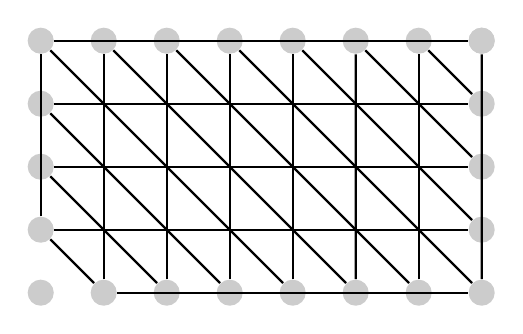
\begin{tikzpicture}
[scale=.8,auto=left,every node/.style={circle,fill=black!20}]
\node (00) at (0,0) {};
\node (10) at (1,0) {};
\node (20) at (2,0) {};
\node (30) at (3,0) {};
\node (40) at (4,0) {};
\node (50) at (5,0) {};
\node (60) at (6,0) {};
\node (70) at (7,0) {};
\node (04) at (0,4) {};
\node (14) at (1,4) {};
\node (24) at (2,4) {};
\node (34) at (3,4) {};
\node (44) at (4,4) {};
\node (54) at (5,4) {};
\node (64) at (6,4) {};
\node (74) at (7,4) {};
\node (71) at (7,1) {};
\node (72) at (7,2) {};
\node (73) at (7,3) {};
\node (74) at (7,4) {};
\node (01) at (0,1) {};
\node (02) at (0,2) {};
\node (03) at (0,3) {};
\Edge(10)(01)
\Edge(20)(02)
\Edge(30)(03)
\Edge(40)(04)
\Edge(50)(14)
\Edge(60)(24)
\Edge(70)(34)
\Edge(71)(44)
\Edge(72)(54)
\Edge(73)(64)
\Edge(01)(71)
\Edge(02)(72)
\Edge(03)(73)
\Edge(10)(14)
\Edge(20)(24)
\Edge(30)(34)
\Edge(40)(44)
\Edge(50)(54)
\Edge(60)(64)
\Edge(10)(70)
\Edge(01)(04)
\Edge(04)(74)
\Edge(74)(70)
\end{tikzpicture}
\item Any kind of graph search algorithm will work starting at $(7,4)$ and ending when one of the coordinates is $2$. I.e. use DFS according to my arbitrary ordering.
\item $$(7,4)\to(0,4)\to(0,1)\to(1,0)\to(1,4)\to(5,0)\to(5,4)\to(7,2)$$
\end{enumerate}
\newpage
\item Break up the graph into strongly connected components. ``Kosaraju's algorithm, Tarjan's algorithm and the path-based strong component algorithm all efficiently compute the strongly connected components of a directed graph" -- pick your favorite one. The new graph, where each node represents a single strongly connected component, is acyclic, so the graph has an odd cycle iff one of its strongly connected components has an odd cycle. Of course, each nontrivial strongly connected component has a cycle, the real question is if one of them has odd length. Given a strongly connected component, we can run a BFS, assigning a value to each of the nodes. We assign the first node in the component $0$, and the next level of nodes (those reachable from the first) a value of $1$, the next level is $0$, and keep repeating. That is, each edge is of length $1$ and each node's assignment is their level $\mod 2$. After we are done labeling the graph, we can go back through and see if two neighbors (nodes that share an edge) have the same label (both $0$ or both $1$). If this is the case, we know that the strongly connected component has an odd cycle. Let the start node be $v$, and the two neighbors $u,w$ with edge $u\to w$. Let the label of $u$ and $w$ be the same. That means that dist$(v,u)$=dist$(v,w)$. From each of these points there must be a path back to $v$ because its strongly connected. Let dist$(w,v)$ be the same parity as dist$(v,w)$ so both even or both odd, this produces as even cycle. But, if we take the dist$(v,u)$, which equals dist$(v,w)$ then add $1$ for dist$(u,w)$ and then add the dist$(w,v)$ that produces an odd cycle. Likewise, if dist$(w,v)$ is not the same parity as dist$(v,w)$ then we already have an odd cycle. Thus we can conclude that if two connected vertices have the same parity $0$ or $1$ then the graph has an odd cycle. If the graph has an odd cycle, there must exist at least one such pair with same parity because it is the equivalent to a back edge in traditional BFS, which must exist because the component has an odd-length cycle, where the two vertices in the back edge must have the same parity because the cycle is of odd length. \\

Now to analyze the runtime. Breaking the graph into strongly connected components is linear. Doing a BFS to label all of the vertices if linear. And the final traversal to find if any pairs have the same parity is also linear, so the total algorithm is linear (although you can combine the BFS with the pair/parity checking, its clearer for the proof to separate them.)
\newpage
\item
\begin{enumerate}
\item An equivalence relation: $(x,x)\in R$, $ \forall x\in S$. $(x,y)\in R \implies (y,x)\in R$, $(x,y)\in R \wedge (y,z)\in R\implies (x,z)\in R$\\
First, $e\sim e$ by definition.\\
Second, $e\sim f \implies f \sim e$. If $e = f$ we have a trivial case (same as above). If $e\neq f$ then there is a simple cycle containing $e$ and $f$. If the cycle contains both $e$ and $f$ then the cycle must contain both $f$ and $e$ and so $f\sim e$.\\
Third, $e\sim f \wedge f\sim g \implies e\sim g$. There is a simple cycle containing $e$ and $f$ and there is a simple cycle containing $f$ and $g$. Because everything is undirected, we can just concatenate the cycles to produce a larger cycle. Splice the cycles together at $f$ and you get a larger cycle (i.e. from $e$ go to $f$ then to $g$ back to $f$ back to $e$ for a bigger cycle). Note that if there are common edges, then you need to pick the right direction to go in, then splice in the cycle with $g$ and then continue back to $e$ (consider the extreme case where $g$ is in the original cycle, we don't have to splice anything). This new cycle contains $e$ and $g$ so $e\sim g$.
\item Biconnected components: $\{AB,BN,NO,OA\}$ $\{DE,EL,LD\}$, \\
$\{LK,KH,HG,GF,FI,IJ,JL\}$, $\{CD\}$, $\{DM\}$\\
Bridges: $BD,DC,DM$, Separating Vertices: $B,D,L$
\item $\{AB,BN,NO,OA\}$: $ABNO$ $\{DE,EL,LD\}$: $DEL$, \\
$\{LK,KH,HG,GF,FI,IJ,JL\}$: $LKHGFIJ$, $\{CD\}$: $CD$, $\{DM\}$: $DM$\\
By contradiction: lets assume that there are two biconnected components that share more than one vertex. That means that they share at least two, lets call then $X,Y$. There must be a path starting at $X$ and ending at $Y$ that doesn't share any edges with the second component, and there must be a path from $Y$ to $X$ in the second component that doesn't share any edges with the first component. Take the first path, and then the second path to see all of these are in the same equivalence class. Next take, the path from $X\to Y$ in the first, and the path from $Y\to X$ (the paths we didn't take the first time), this produces another equivalence class, but it must be the same as the previous because both halves belong to it individually. Because all the edges are in the same equivalence class, there are not two biconnected components in the graph. Therefore, two biconnected components cannot share more than one vertex (aka they must be disjoint or share one vertex, there are examples of both of these cases earlier).
\item Collapse each biconnected components of the graph. Keep the separating nodes. There cannot possibly be a cycle in this new graph because each of the components doesn't share a cycle with other components, or else they would be in the same component. Therefore, the collapsed graph must be a tree.
\item If the root of DFS has more than one child, then it has two tree edges to distinct biconnected components, so its a separating vertex. If the root node of the DFS is a separating vertex, then is connects two otherwise separate biconnected components together, therefore it must have at least two children, two vertices that are reachable from the root.
\item If $v$ is a separating vertex, then removing it from the graph disconnects it. Therefore, if we preform a BFS, when we get to $v$, there must be one subtree that is reachable from $v$ that doesn't connect back to the graph, (if there didn't exist such a child then each of $v$'s children would still be connected if $v$ were removed). Lets call this child $v'$. $v'$ or its children cannot have a back edge to a proper ancestor of $v$ -- if it did, then removing $v$ would not separate that tree (which we know it has to do). \\
Given that $v$ has a child $v'$ that doesn't have a back edge to a proper ancestor of $v$, we can conclude that $v$ is a separating vertex. Because $v'$ an none of its children have back edges to a proper ancestor of $v$, there are no cycles in the subgraph EXCEPT if the cycle includes $v$ and none of $v's$ ancestors. If the cycle includes $v$, and none of its ancestors, then removing $v$ will remove both edges to $v$ and detach the cycle from the rest of the graph, if it has no cycle, then removing $v$ will also detach the subtree. Thus, $v$ is a separating vertex.\\
\item Preform a DFS is linear time to label each vertex with its pre and post numbers. While exploring all of a node's children, save each of their low numbers (which must be computed before each vertex's post visit). Upon post-visiting this vertex, take the minimum of its pre number and each of its children's low numbers. This is the recursive step. but we need base cases. If you get to a vertex and it has a back edge, i.e. its pre number is greater than the next vertex but the next vertex's post number hasn't been set yet, then assign to it the minimum of its pre number, the back edge's target vertex's pre number and each of its children's low numbers. Next, if a vertex has no children, its low number is its pre number. This can all be computed in a single DFS, linear time.
\item Preform another DFS, for each vertex, $v$, if $v$'s low number is its pre number, then $v$ is a separating vertex. Group all edges between vertices of the same low numbers together -- these are the biconnected components. Edges between separating vertices are bridges. You can preform another DFS after calculating low numbers to group all of these components together. I.e. if the vertex's child has a different low number than the vertex, both are separating vertices and the edge between them is a bridge, etc.
\end{enumerate}
\newpage
\begin{enumerate}
\item{4.1(a)} We mark visited nodes with $(V)$
\begin{displaymath}
\begin{array}{|c|c|c|c|c|c|c|c|}
\hline
A & B&C&D&E&F&G&H\\
\hline
0 & \infty & \infty & \infty & \infty & \infty & \infty & \infty \\
\hline
0 (V)& 1 & \infty & \infty & 4 & 8 & \infty & \infty \\
\hline
0 (V)& 1 (V) & 3 & \infty & 4 & 7 & 7 & \infty \\
\hline
0 (V)& 1 (V) & 3 (V)& 4 & 4 & 7 & 5 & \infty \\
\hline
0 (V)& 1 (V) & 3 (V)& 4 (V) & 4 & 7 & 5 & 8 \\
\hline
0 (V)& 1 (V) & 3 (V)& 4 (V) & 4 (V)& 7 & 5 & 8 \\
\hline
0 (V)& 1 (V) & 3 (V)& 4 (V) & 4 (V)& 6 & 5 (V) & 6 \\
\hline
0 (V)& 1 (V) & 3 (V)& 4 (V) & 4 (V)& 6 (V) & 5 (V) & 6 \\
\hline
0 (V)& 1 (V) & 3 (V)& 4 (V) & 4 (V)& 6 (V) & 5 (V) & 6 (V) \\
\hline
\end{array}
\end{displaymath}
\item{4.1(b)}
\Tree[.A [.E ]
         [.B 
			 [.C [.D ]
                           [.G [.F ]
                                [.H ]
                            ]
			 ]	
		]
	]
\item{4.2(a)}
\begin{displaymath}
\begin{array}{|c|c|c|c|c|c|c|c|c|c|}
\hline
S&A & B&C&D&E&F&G&H&I\\
\hline
0 & \infty & \infty & \infty & \infty & \infty & \infty & \infty & \infty  & \infty \\
\hline
0 & 7 & \infty & 6 & \infty & 6 & 5 & \infty & \infty  & \infty \\
\hline
0 & 7 & 11 & 5 & 8 & 6 & 4 & \infty & 9  & \infty \\
\hline
0 & 7 & 11 & 5 & 7 & 6 & 4 & 9 & 7  & \infty \\
\hline
0 & 7 & 11 & 5 & 7 & 6 & 4 & 8 & 7  & 8 \\
\hline
0 & 7 & 11 & 5 & 7 & 6 & 4 & 8 & 7  & 7 \\
\hline
\end{array}
\end{displaymath}
\item{4.2(b)}
\Tree[.S [.A 
			[.C [.D ]]
			[.B 
				[.H [.G [.I ]]]]
			]
		 [.E [.F ]]
		]
\item{4.4}
\[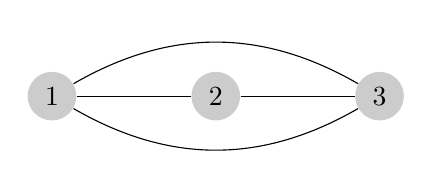
\begin{tikzpicture}[scale=.8,auto=left,every node/.style={circle,fill=black!20},
x=1.3cm, y=1cm,
    every edge/.style={
        draw,
        }
]

\node (1) at (2,0) {1};
\node (2) at (4,0) {2};
\node (3) at (6,0) {3};
\path
		(1) edge (2)
		(2) edge (3)
		(1) edge[bend left] (3)
		(1) edge[bend right] (3)
	;
\end{tikzpicture}\]
A DFS starting at $1$ going to $2$ then $3$ will find a cycle of length $3$. Upon popping off the stack back to $1$, it will see that $3$ is already visited, and so it won't find the cycle of length $2$, so the algorithm doesn't work. In general, it ignores different paths through cycles because DFS will still not look at a node that has already been expanded and visited.
\end{enumerate}
\end{enumerate}
\end{document}
